\documentclass[preprint,12pt, a4paper]{elsarticle}

\usepackage{amsmath}
\usepackage{amssymb}
\usepackage{array}
\usepackage{booktabs}
\usepackage{color}
\usepackage{float}
\usepackage{graphicx}
\usepackage{ifpdf}
\usepackage[utf8]{inputenc}
\usepackage{keyval}
\usepackage{lineno}
\usepackage{listings}
\usepackage{longtable}
\usepackage{moresize}
\usepackage{multirow}
\usepackage{paralist}
\usepackage{rotating}
\usepackage{soul}
\usepackage{srcltx}
\usepackage{url}
\usepackage{xcolor}
\usepackage{xspace}
\usepackage{wrapfig}
\usepackage{subfig}
\usepackage{tikz}
\usepackage[export]{adjustbox} % http://ctan.org/pkg/adjustbox

\definecolor{listinggray}{gray}{0.95}
\definecolor{darkgray}{gray}{0.7}
\definecolor{commentgreen}{rgb}{0, 0.4, 0}
\definecolor{darkblue}{rgb}{0, 0, 0.6}
\definecolor{purple}{rgb}{0.6, 0, 0.6}
\definecolor{middleblue}{rgb}{0, 0, 0.75}
\definecolor{darkred}{rgb}{0.4, 0, 0}
\definecolor{brown}{rgb}{0.5, 0.5, 0}
\definecolor{dkgreen}{rgb}{0,0.5,0}
\definecolor{orange}{rgb}{1,.5,0}
\definecolor{dandelion}{cmyk}{0,0.29,0.84,0}

\usepackage[normalem]{ulem}
\makeatletter
\def\cyanuwave{\bgroup \markoverwith{\lower3.5\p@\hbox{\sixly \textcolor{cyan}{\char58}}}\ULon}
\def\reduwave{\bgroup \markoverwith{\lower3.5\p@\hbox{\sixly \textcolor{red}{\char58}}}\ULon}
\def\blueuwave{\bgroup \markoverwith{\lower3.5\p@\hbox{\sixly \textcolor{blue}{\char58}}}\ULon}
\font\sixly=lasy6 % does not re-load if already loaded, so no memory problem.
\makeatother

\def\BibTeX{{\rm B\kern-.05em{\sc i\kern-.025em b}\kern-.08em
    T\kern-.1667em\lower.7ex\hbox{E}\kern-.125emX}}

% Generate circled numbers
\newcommand*\circled[1]{\tikz[baseline=(char.base)]{
    \node[shape=circle,draw,inner sep=1pt] (char) {#1};}}
\newif\ifdraft{}
%\drafttrue{}

\ifdraft{}
  \newcommand{\amnote}[1]{ \textcolor{blue} { ***andrem: #1 }}
  \newcommand{\jhanote}[1]{ {\textcolor{red} { ***shantenu: #1 }}}
  \newcommand{\mtnote}[1]{ {\textcolor{orange} { ***matteo: #1 }}}
\else
  \newcommand{\amnote}[1]{}
  \newcommand{\jhanote}[1]{}
  \newcommand{\mtnote}[1]{}
\fi

\newcommand{\apples}{AppLeS\xspace}
\newcommand{\bj}{BigJob\xspace}
\newcommand{\computeunit}{Compute-Unit\xspace}
\newcommand{\computeunits}{Compute-Units\xspace}
\newcommand{\cloud}{cloud\xspace}
\newcommand{\clouds}{clouds\xspace}
\newcommand{\cc}{c\&c\xspace}
\newcommand{\CC}{C\&C\xspace}
\newcommand{\computedataservice}{Compute-Data Service\xspace}
\newcommand{\cu}{CU\xspace}
\newcommand{\cus}{CUs\xspace}
\newcommand{\dataunit}{Data-Unit\xspace}
\newcommand{\dataunits}{Data-Units\xspace}
\newcommand{\du}{DU\xspace}
\newcommand{\dus}{DUs\xspace}
\newcommand{\mrmg}{MR-Manager\xspace}
\newcommand{\MW}{master-worker\xspace}
\newcommand{\numrep}{8 }
\newcommand{\panda}{PanDA\xspace}
\newcommand{\pilot}{Pilot\xspace}
\newcommand{\pilots}{Pilots\xspace}
\newcommand{\pilotjob}{Pilot-Job\xspace}
\newcommand{\pilotjobs}{Pilot-Jobs\xspace}
\newcommand{\pilotcompute}{Pilot-Compute\xspace}
\newcommand{\pilotcomputes}{Pilot-Computes\xspace}
\newcommand{\pilotdata}{Pilot-Data\xspace}
\newcommand{\pilotdataservice}{Pilot-Data Service\xspace}
\newcommand{\pilotcomputeservice}{Pilot-Compute Service\xspace}
\newcommand{\prop}[1]{\textit{#1}\xspace}
\newcommand{\pilotmapreduce}{PilotMapReduce\xspace}
\newcommand{\pstar}{P*\xspace}
\newcommand{\pd}{PD\xspace}
\newcommand{\pj}{PJ\xspace}
\newcommand{\pjs}{PJs\xspace}
\newcommand{\pds}{Pilot Data Service\xspace}
\newcommand{\samplenum}{4 }
\newcommand{\su}{SU\xspace}
\newcommand{\sus}{SUs\xspace}
\newcommand{\schedulableunit}{Schedulable Unit\xspace}
\newcommand{\schedulableunits}{Schedulable Units\xspace}
\newcommand{\tmax}{\(T_{max}\)}
\newcommand{\tc}{\(T_{C}\)}
\newcommand{\tcnsp}{\(T_{C}\)}
\newcommand{\vocab}[1]{\textbf{#1}\xspace}

\newcommand{\B}[1]{\textbf{#1}\xspace}
\newcommand{\C}[1]{\textsc{#1}\xspace}
\newcommand{\F}[1]{\textbf{FIXME\@: #1}\xspace}
\newcommand{\I}[1]{\textit{#1}\xspace}
\newcommand{\T}[1]{\texttt{#1}\xspace}

\newcommand{\impterm}[1]{\texttt{#1}\xspace}

% System names
\newcommand{\bw}{\I{Blue\,Waters}}
\newcommand{\stampede}{\I{Stampede}}
\newcommand{\comet}{\I{Comet}}
\newcommand{\titan}{\I{Titan}}

% Latex Fu
\newcommand{\UPP}{\vspace*{-2.0em}}
\newcommand{\UP}{\vspace*{-1.0em}}
\newcommand{\up}{\vspace*{-0.5em}}

% Paper specific Macro's
\newcommand{\ru}{$RU$\xspace}
\newcommand{\ttc}{$ttc$}
\newcommand{\ttca}{$ttc_a$}

% Table multirows
\newcommand{\mr}[1]{\multirow{2}{*}{#1}}%
\newcommand{\mc}[2]{\multicolumn{#1}{l}{#2}}

\lstdefinestyle{myListing}{
  frame=single,   
  backgroundcolor=\color{listinggray},  
  %float=t,
  language=C,       
  basicstyle=\ttfamily \footnotesize,
  breakautoindent=true,
  breaklines=true
  tabsize=2,
  captionpos=b,  
  aboveskip=0em,
  belowskip=-2em,
}      

\lstdefinestyle{myPythonListing}{
  frame=single,   
  backgroundcolor=\color{listinggray},  
  %float=t,
  language=Python,       
  basicstyle=\ttfamily \footnotesize,
  breakautoindent=true,
  breaklines=true
  tabsize=2,
  captionpos=b,  
}

% This is now the recommended way for checking for PDFLaTeX:
\ifpdf{}
  \DeclareGraphicsExtensions{.pdf, .jpg, .tif}
\else
  \DeclareGraphicsExtensions{.eps, .jpg, .ps}
\fi

\tolerance=1000
\hyphenpenalty=10


\journal{SoftwareX}

\begin{document}
\begin{frontmatter}

% \title{Title/Name of your software}
\title{RADICAL Cybertools}

\author{A. Author}
\address{Your institute, some address}

\author{B. Author}
\address{Your institute, some address}

\author{C. Author}
\address{Your institute, some address}

\author{D. Author}
\address{Your institute, some address}

\begin{abstract}
Ca. 100 words
\end{abstract}

\begin{keyword}
%% keywords here, in the form: keyword \sep keyword
keyword 1 \sep keyword 2 \sep keyword 3

%% PACS codes here, in the form: \PACS code \sep code

%% MSC codes here, in the form: \MSC code \sep code
%% or \MSC[2008] code \sep code (2000 is the default)

\end{keyword}

\end{frontmatter}

\linenumbers{}

% {\em The manuscript must be submitted in single column. The following
% constraints apply:
% \begin{enumerate}
%   \item Word count: max. 3000. Excluding: title, authors, affiliations,
%         references, metadata tables; Including: abstract, running text,
%         captions, footnotes.
%   \item Max. 6 figures.
%   \item The manuscript must have line numbers.
%   \item At least one of the two mandatory metadata tables located at the
%         end of the article template must be filled in and included in the
%         manuscript.
%   \item To submit your code/software you can: Point to an external location
%         (repository, archive, etc.) where the code is publicly available.
%         Clearly mark the address to retrieve the code in the metadata
%         tables included in the manuscript.
% \end{enumerate}}


% ---------------------------------------------------------------------------
% Section I
% ---------------------------------------------------------------------------
\section{Motivation and significance}\label{sec:motivation}

% {\em Guidelines for the authors:
% \begin{enumerate}
%   \item Introduce the scientific background and the motivation for
%         developing the software.
%   \item Explain why the software is important, and describe the exact
%         (scientific) problem(s) it solves.
%   \item Indicate in what way the software has contributed (or how it will
%         contribute in the future) to the process of scientific discovery;
%         if available, this is to be supported by citing a research paper
%         using the software.
%   \item Provide a description of the experimental setting (how does the
%         user use the software?).
%   \item Introduce related work in literature (cite or list algorithms used,
%           other software etc.).
% \end{enumerate}}

The design of distributed systems to support scientific computing has never
been more challenging. Unprecedented diversity in application requirements,
and disruptive changes in the resources and technology landscapes, intermix
with new discovery modalities and need for scalable computing.

Set against this dynamic landscape, two critical question must be addressed:
How can middleware be designed and implemented to meet the collective
challenges of scale, new and diverse functionality, and usability? How can
critical middleware components be designed to be sustainable software
implementations while being forward looking and enable innovative
capabilities?

RADICAL-Cybertools (RCT) are a set of systems developed to address these
challenges.  RCT are building blocks, which can be used as a stand-alone
system, or integrated with other RCT, or third-party tools to enable diverse
functionalities. RCT offer several innovative features to support the design
and implementation of middleware.

This paper takes a software perspective to present the overarching
architectural paradigm of RCT, discussing the design and implementation of
two cybertools: RADICAL-Pilot and Ensemble-Toolkit (EnTK). We outline the
direct impact that RCT are having on domain sciences, focusing the discussion
on architectural and design paradigms of middleware for scientific computing.
In this way, we show how RCT further the ``state-of-theory'' and practice of
scientific computing.


% ---------------------------------------------------------------------------
% Section II
% ---------------------------------------------------------------------------
\section{Software description}\label{sec:description}

% {\em Describe the software in as much as is necessary to establish a
% vocabulary needed to explain its impact.}

The RADICAL Cyberinfrastructure tools (RCT)~\cite{web-rct} is a software
suite composed of three main components: RADICAL-SAGA
(RS)~\cite{merzky2015saga}, RADICAL-Pilot (RP)~\cite{merzky2018using} and
RADICAL-Ensemble Toolkit (EnTK)~\cite{balasubramanian2018harnessing}.

RS is a Python implementation of the OGF GFD.90 SAGA
standard~\cite{goodale2006saga}, a high-level interface to access distributed
infrastructure components like job schedulers, file transfer and resource
provisioning services. RS enables interoperability across heterogeneous
distributed infrastructures, improving on their usability and enhancing the
sustainability of services and tools.

RP is a Python implementation of the pilot paradigm and architectural
pattern~\cite{turilli2018comprehensive}. Pilot systems enable users to submit
pilot jobs to computing infrastructures and then use the resources acquired
by the pilot to execute one or more tasks. These tasks are directly scheduled
via the pilot, without having to queue in the infrastructure batch system. RP
focuses on High Performance Computing (HPC), enabling the execution of
heterogeneous workloads comprised of one or more scalar, MPI, OpenMP,
multi-process, and multi-threaded tasks. These tasks can be executed on CPUs,
GPUs and other accelerators, on the same pilot or across multiple pilots.

EnTK supports the concurrent or sequential execution of an ensemble of tasks
or pipelines of tasks. EnTK promotes ensembles to a high-level programming
abstraction, providing a programming interface and execution model specific
to ensemble-based applications. EnTK is engineered for scale and a diversity
of computing platforms and runtime systems, agnostic of the size, type and
coupling of the tasks comprising the ensemble.

RCT are designed to work both individually and as an integrated system. This
requires a ``Building Block'' approach to their design and development, based
on applying the traditional notions of modularity at system level. The
Building Block approach derives from the work on Service-oriented
Architecture and its Microservice variants, and the component-based software
development approaches where computational and compositional elements are
explicitly
separated~\cite{batory1992design,garlan1995architectural,lenz1988software,clemens1998component,schneider2000components}.
AirFlow, Oozie, Azkaban, Spark Streaming, Storm, or Kafka are examples of
tools that have a design consistent with the building blocks approach.

In our adaptation, the Building Block approach is based on four
well-understood principles: self-sufficiency, interoperability,
composability, and extensibility. This approach does not reinvent modularity,
it applies it at system level to enable composability among independent
software systems. As an abstraction, modularity enables separation of
concerns by encapsulating discrete functions into semantic units exposed by
means of a dedicated interface. As such, modularity can be used at function
or method level, depending on the programming paradigm and the facilities
offered by programming languages, or at system-level, depending on the
interface exposed by each system.

% ---------------------------------------------------------------------------
\subsection{Software Architecture}\label{ssec:architecture}

% {\em Give a short overview of the overall software architecture; provide a
% pictorial component overview or similar (if possible). If necessary provide
% implementation details.}

All RCT are stand-alone, distributed systems. Architecturally, each tool
consists of one or more subsystems, each with several components. Components
are isolated into separate processes and some components are used only in
specific deployment scenarios, depending on both application requirements and
resource capabilities. Components are stateless and some of them can be
instantiated concurrently to simultaneously manage multiple entities, like
workflows, workloads, tasks or pilots. This enables scaling of throughput and
tolerance to component failure.

Concurrent components are coordinated via a dedicated communication mesh,
which introduces runtime and infrastructure-specific overheads, but improves
overall scalability of the system and lowers component complexity. Components
can have different implementations; configuration files can tailor each RCT
to specific resources types, workloads, or scaling requirements. Components
exchange data about the entities specific to each RCT and data about the
state of the components and subsystems. Each type of data has dedicated
modules and communication channel, separating communication from coordination
while making explicit states and events of each entity.

Ref.~\cite{merzky2015saga} details RADICAL-SAGA architecture and
capabilities. Here, we focus on RP and EnTK, first introducing each system
individually, then showing how RCT as a whole can be composed to serve
diverse use cases.

% ------------
\subsubsection{RADICAL-Pilot}\label{sssec:arch_rp}

RP implements two main abstractions: Pilot and Compute Unit (CU). Pilots and
CUs abstract away specificities of resources and workloads, making it
possible to schedule workloads either concurrently or sequentially on
resource placeholders. Pilots are placeholders for computing resources, where
resources are represented independent from architecture and topological
details. CUs are units of work (i.e., tasks), specified as an application
executable alongside its resource and execution environment requirements.
Note that a task is not a function, method, thread or process but a program
that can be run as a self-contained executable.

Fig.~\ref{fig:archs}a depicts RP's architecture with two subsystems (white
boxes) and several components (purple and yellow boxes). In each subsystem,
purple components are responsible for pilots and units while yellow
components manage the communication among RP components. Subsystems can
execute locally or remotely, communicating and coordinating over TCP/IP\@,
and enabling multiple deployment scenarios. For example, users can run Client
locally, and distribute MongoDB and one or more instances of Agent on remote
computing infrastructures. Alternatively, users can run all RP components on
a local or remote resource.

\begin{figure}
    \centering
    \subfloat[ ]{{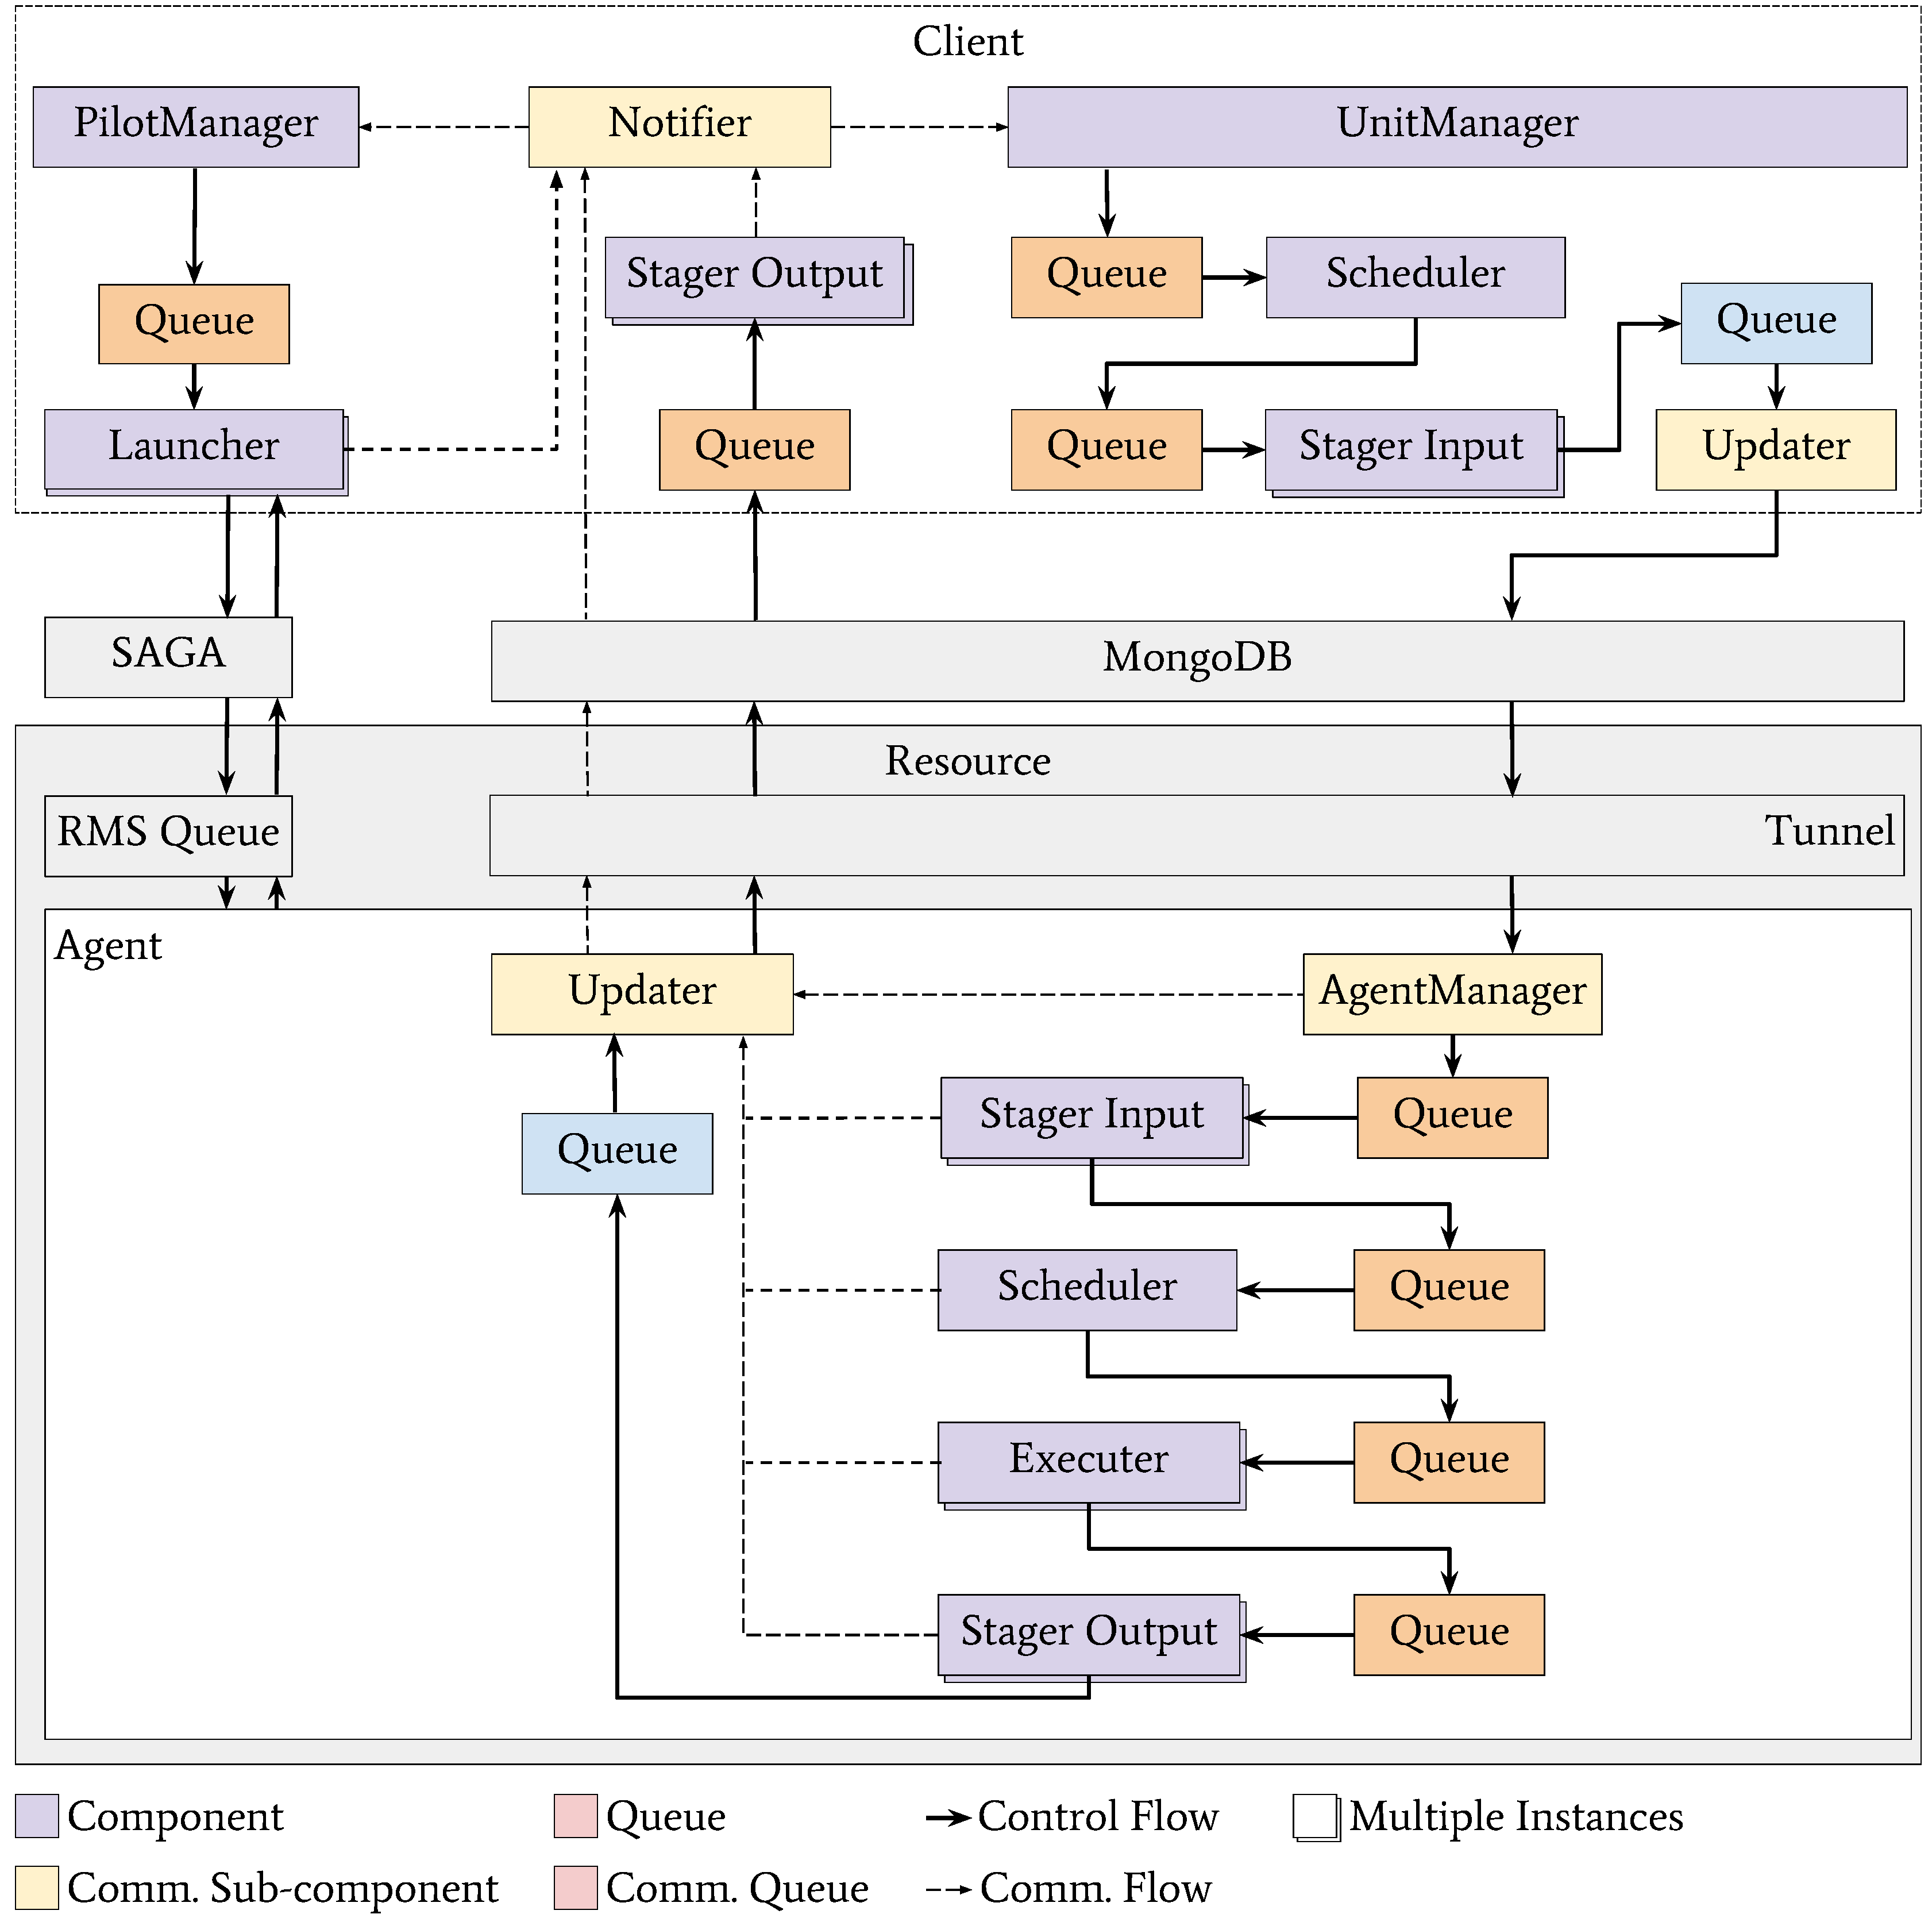
\includegraphics[width=0.58\textwidth]{figures/arch_rp.pdf} }}
    \qquad
    \subfloat[ ]{{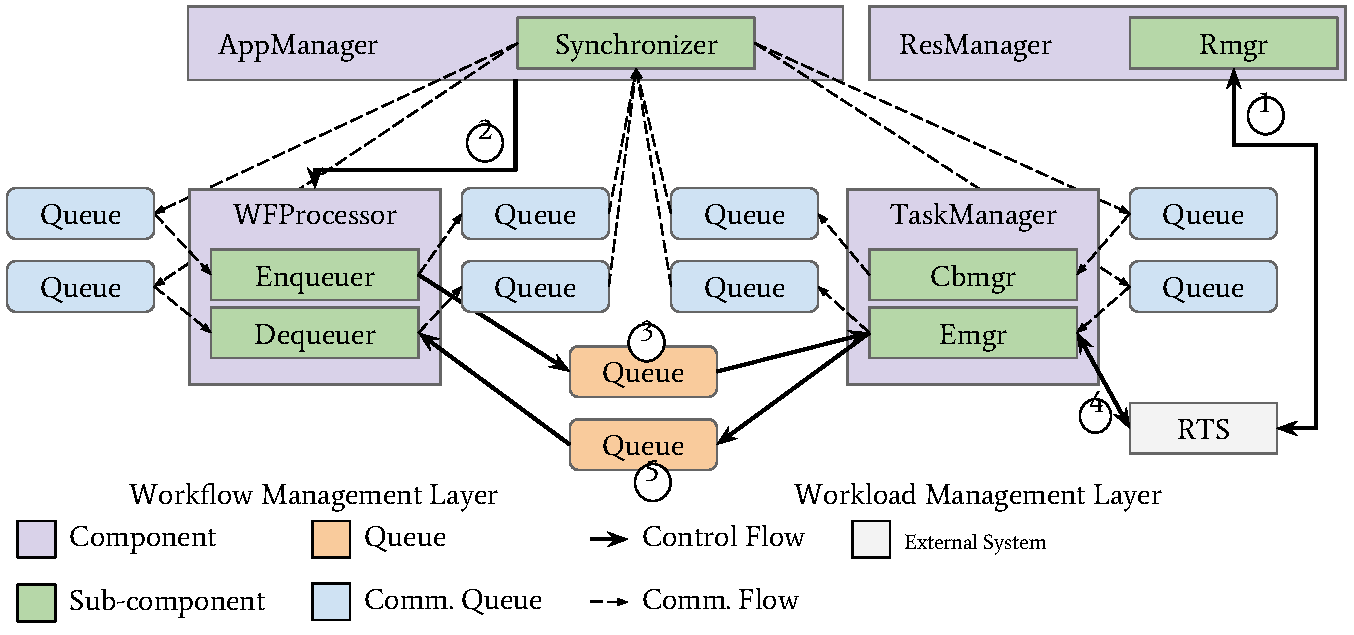
\includegraphics[width=0.32\textwidth]{figures/arch_entk.pdf} }}
    \caption{Caption. \mtnote{TODO\@: Fix EnTK AppManager}}\label{fig:archs}
\end{figure}

The first subsystem, called Client, has two main components designed to
manage either pilots or units: PilotManager and UnitManager. PilotManager has
a main component called `Launcher'. The Launcher uses resource configuration
files to define the number, placement, and properties of the Agent's
components of each Pilot. Currently, configuration files are made available
for all the HPC machines of the Extreme Science and Engineering Discovery
Environment (XSEDE), Blue Waters at the National Center For supercomputing
Applications (NCSA), Cheyenne at NCAR-Wyoming Supercomputing Center (NWSC),
and Rhea, Titan and Summit at the Oak Ridge National Laboratory (ORNL). Users
can provide new files or alter existing configuration parameters at runtime,
both for a single pilot or a whole RP session.

UnitManager has two main components: Scheduler and Stager Input. Scheduler
schedules compute units onto one or more pilots, available on one or more
resources. This enables late binding of units to resources, depending on
their availability: units are bound to resources that satisfy their execution
requirements only when these resources are actually available. The second
component of UnitManager is Stager Input. Units may need input files for
their execution, this module takes care to distribute these files to the
resources on which each unit has been scheduled.

The second subsystem of RP is called Agent and has four main components: one
Stager Input and Stager Output for staging input and output data of compute
units, Scheduler and Executer to schedule compute units on a pilot resources
and execute those units on them. Multiple instances of the Stager and
Executer components can coexist in a single Agent. Depending on the
architecture of the resource, the Agent's components can individually be
placed on cluster head nodes, MOM nodes, compute nodes, virtual machines, or
any combination thereof. ZeroMQ communication bridges connect the Agent
components, creating a network to support the transitions of the units
through components.

Data management \ldots\mtnote{Andre to write this paragraph about the
architectural specifics of data management in RP, mentioning Stager Output in
Client.}

Each component of each subsystem of RP has a dedicated queue. Orange queue in
Fig.~\ref{fig:archs}a are dedicated to pilots and unit entities while blue
queues to the messages exchanged by the components dedicated to
communication. Queuing entities enables managing them in bulk so to obtain
performance at scale in a distributed systems. Further, queuing entities
enables the use of concurrent components when using multiple physical
supports (e.g., work nodes) or when leveraging component concurrency for
performance optimization.

\mtnote{Andre: Introduce MongoDB and the role it plays for communication and
coordination? I know it is on its way out but at the moment it is in the
diagram.}

% ------------
\subsubsection{RADICAL Ensemble Toolkit}\label{sssec:arch_entk}

EnTK implements three main abstractions: task, stage and pipeline. Tasks
contain information regarding an executable, its software environment and its
data dependences. Stages are set of tasks where tasks have no mutual
dependences and can therefore execute concurrently, depending on resource
availability. Pipelines are lists of stages where a stage \(i\) can be
executed only after stage \(i-1\) has been executed.

The task abstraction identifies an executable as a program, not as an
instruction of a program. This is important: EnTK enables concurrent and
sequential execution at program-level, not at instruction level.
Instruction-level parallelism is still possible within each program run by an
EnTK task, enabling concurrent execution of multi-threaded, multi-process and
MPI programs. Note that. at the moment, EnTK requires a runtime system (RTS)
that support the same task abstraction.

Fig.~\ref{fig:archs}b shows the architecture of EnTK. The EnTK system (white)
has three components (purple), each with subcomponents dedicated to the
management of EnTK's entities (green) or coordination of the entities'
execution (yellow). The three components are AppManager, WFProcessor and
TaskManager that enable workflow specification, workflow execution
management, and workload management.

AppManager exposes an API for the development of ensemble-based applications
in terms of tasks, stages and pipelines, and for specifying resource
requirements for the application execution. AppManager initializes EnTK and
holds the global state of the application at runtime. AppManager is the sole
stateful component of EnTK, allowing to restart other components upon
failure, without interrupting the execution of the ensemble-based
application.

WFProcessor uses the Enqueue and Dequeue subcomponents to queue and dequeue
tasks pulled from AppManager. TaskManager uses ExecManager to schedule tasks
on the RTS and keep track of the state of each task during execution.
TaskManager users ResManageer as an interface to the chosen RTS. RTS have to
provide capabilities to acquire resources and schedule tasks on those
resources for execution. ResManager isolates RTS from EnTK, enabling
restarting of the RTS without loosing information about tasks that have been
already executed. Currently, EnTK support only RADICAL-Pilot as RTS but it is
designed to use other task-based RTS as, for example, Coasters or HTCondor.

% ---------------------------------------------------------------------------
\subsection{Software Functionalities}\label{ssec:functionalities}

% {\em Present the major functionalities of the software.}

% SAGA
Given the heterogeneity of distributed infrastructures, SAGA provides a much
needed interoperability layer that lowers the complexity and improves the
simplicity of using distributed infrastructure whilst enhancing the
sustainability of distributed applications, services and
tools.\mtnote{probably not to be included as SAGA has been already described
in a standalone SoftwareX publication.}

% RP
As a runtime system, RP offers an API to describe both pilots and CUs,
alongside classes and methods to manage acquisition of resources, scheduling
of CUs on those resources, and the staging of input and output files.
Reporting capabilities update the user about ongoing executions and profiling
capabilities enable detailed postmortem analysis of workload executions and
runtime behavior.

RP enables the execution of tasks with several dimensions of heterogeneity on
one or more pilots instantiated on one or more resources. The defining
capability of a pilot system is to decouple resource acquisition from task
execution. Infrastructures exposing resources via a batch system allow users
to submit their tasks as jobs. Jobs wait in the batch system's queue and when
the requested resources became available for the requested amount of time, a
job is scheduled for execution. Thus, each task of a multi-task application
has to wait in the batch system's queue to be executed, incurring in delays
that can become rapidly unfeasible.

Pilot systems allow for queuing a single job via the batch system and, once
this job becomes active, it executes a system application that enables the
direct scheduling of tasks on the acquired resources, without waiting in the
batch system's queue. In this way, pilot systems can enable high throughput
computing (HTC) on infrastructures designed to enable high performance
computing (HPC). Note that pilot systems do not game the HPC infrastructure:
pilot jobs are bound by the required resources and wait in the queue as every
other job, therefore abiding to the system usage policies.

RP offers four unique features when compared to other pilot systems or tools
that enable the execution of multi-task applications on HPC systems: (1)
concurrent execution of heterogeneous tasks on the same pilot; (2) support of
all the major HPC batch systems; (3) support of more than twelve methods to
launch tasks; and (4) a general purpose architecture. RP can execute single
or multi core tasks within a single compute node, or across multiple nodes,
isolating the execution of each tasks into a dedicated process and enabling
concurrent execution of heterogeneous tasks by design.

% EnTK
EnTK is a workflow engine specifically designed to execute ensemble-based
applications. These applications are composed by ensemble of tasks that may
have dependences both among tasks and ensembles. These dependences express a
relationship of priority at execution time. These dependences may be
determined by input/output data and control flow requirements: For example,
two tasks may have to be executed sequentially when the output of the first
task is the input of the second task; and two tasks (or ensembles) may have
to be executed sequentially when the output of the first tasks determines
whether executing the second task is of interest.

Consistently, EnTK provides adaptive capabilities and dedicated constructs to
pause, resume and stop pipelines at execution time. Adaptive applications
change the ensemble specifications at runtime, creating new pipelines, stages
and tasks, or changing the properties of those already described. Further,
pipelines and stages can be paused while waiting to perform \textit{ad hoc}
computations. This enable the implementation of high-level application
patterns as, for example, simulation-analysis, replica exchange and \ldots

% Execution Model

\mtnote{Describe BB and individual + aggregated execution models}


% ---------------------------------------------------------------------------
% \subsection{Sample code snippets analysis (optional)}\label{ssec:code}


% ---------------------------------------------------------------------------
% Section III
% ---------------------------------------------------------------------------
\section{Illustrative Examples}\label{sec:examples}

% {\em Provide at least one illustrative example to demonstrate the major
% functions.

% Optional: you may include one explanatory video that will appear next to
% your article, in the right hand side panel. (Please upload any video as a
% single supplementary file with your article. Only one MP4 formatted, with
% 50MB maximum size, video is possible per article. Recommended video
% dimensions are 640 x 480 at a maximum of 30 frames/second. Prior to
% submission please test and validate your .mp4 file at $
% http://elsevier-apps.sciverse.com/GadgetVideoPodcastPlayerWeb/verification$.
% This tool will display your video exactly in the same way as it will appear
% on ScienceDirect.).}

\mtnote{Use a use case that requires a bag of heterogeneous tasks. Show how
this example can become one state of a workflow and how this workflow is
supported by EnTK\@. REPEX, EXTASY candidate examples.}

Multiple scientific domains can benefit from executing many-task applications
at scale, especially at the scale enabled by leadership-class HPC
machines~\cite{raicu2008many,iosup2011performance}. Independent of the domain
for which these applications are developed, their execution requires to run a
single task, a bag of tasks, or a workflow. It is important to note that, in
this context, task refers to a program in the form of a self-contained
executable like, for example, GROMACS, NAMD, AMBER, AthenaMP, SPECFEM and
many others. Multi-task applications requires to concurrently run multiple
instances of programs, using scale to reduce the total time to completion of
the whole execution.

As seen in Sec.~\ref{sec:description}, RCT support the execution of a single
task, a bag of tasks, and workflows expressed as a set or a sequence of
pipelines with stages and tasks. Because of the separation between manging
the concurrent and consecutive execution of tasks and the computation
performance by each task, RCT support multi-task application independent from
the scientific domain in which they are used. From RCT point of view, every
execution reduces exclusively to manging the execution of single or multiple
sets of black boxes.

RADICAL-Pilot (RP) executes set of tasks. The degree of concurrency of the
execution depends on the amount of available resources. Consider for example
a many-task application for the simulation of molecular dynamics with an
ensemble of 128 simulations, each requiring 24 CPU cores as those used in
Ref.~\cite{balasubramanian2016extasy}. The user can use RP API to describe a
pilot job with 3072 cores (Code~\ref{code:pilot}), 128 tasks
(Code~\ref{code:units}) and two managers to coordinate the acquisition of the
pilot resources via RADICAL-SAGA on an HPC machine (Code~\ref{code:pmgr}) and
the execution of the 128 tasks on those resources (Code~\ref{code:umgr}).

Fig.~\ref{fig:archs}a's numbers illustrate the resource acquisition and task
execution process. PilotManager queues the pilot description on one of the
available Launcher in RP client (Fig.~\ref{fig:archs}a.1). That Launcher uses
RADICAL-SAGA to schedule the pilot as a job on the target resource via the
resource's batch System (Fig.~\ref{fig:archs}a.2--3). The pilot job waits in
the resource management system queue and, once scheduled, bootstraps the
pilot's AgentMnager and Updater (Fig.~\ref{fig:archs}a.4). AgentManager forks
the StagerInput, Scheduler, Executor and StagerOutput components and the
Updater notifies RP Client's Notifier that RP Agent is ready to execute tasks
(Fig.~\ref{fig:archs}a.5--7).

Upon notification, UnitManager queues all the available tasks onto RP
Client's Scheduler that, in turns, queues those tasks into the StagerInput,
depending on the chosen scheduling algorithm (Fig.~\ref{fig:archs}a.8--10).
If required, StagerInput stages the tasks' input files to the target resource
and then tasks are queued to the Updater and passed to the chosen RP Agent's
AgentManager (Fig.~\ref{fig:archs}a.11--13). At that point, tasks are passed
to a StagerInput where input files are linked and made available to each
task, and then queued to the RP Agent's Scheduler (Fig.~\ref{fig:archs}a.14).
Scheduler places tasks on suitable partitions of the pilot's resources and
then queue to the Executor so that, when those partitions of resource becomes
available, tasks are executed (Fig.~\ref{fig:archs}a.14). Executor sets up
the environment required by each task and then forks each task for execution
(Fig.~\ref{fig:archs}a.14). This is why tasks are black boxes to RP\@; also
note that Scheduler and Executor can place and fork heterogeneous tasks,
i.e., task requiring different type and amount core/GPUs and different
execution time.

RP cannot manage dependences among tasks. For RP, every task is assumed to be
ready for execution. For example, assume a typical simulation-analysis
workflow for molecular dynamics with a simulation stage and an analysis stage
that depends upon the completion of the simulation stage. Each stage consists
of a set of tasks but RP cannot distinguish between the two. EnTK enables
this distinguishing: each stage is submitted to RP for execution, respecting
their priority relation.

Fig.~\ref{fig:archs}b's numbers illustrate the execution of workflows in
EnTK\@. Users instantiate an AppManager (Code~\ref{code:appnam}), define a
set of resources on which to run their workflow (Code~\ref{code:entk-res}),
describe that workflow in terms of pipelines, stages and tasks
(Code~\ref{code:pst}) and execute it (Code~\ref{code:pst}). AppManager passes
a copy of the workflow description to WFProcessor that, based on the
priorities between stages and tasks, uses Enquerer to queue tasks that are
ready for execution to the task manager (Fig.~\ref{fig:archs}b.1--2).
Meanwhile, ResManager users the chosen runtime system to acquire the
requested resources (Fig.~\ref{fig:archs}b.3) and, once available,
TaskManagers uses those resources to execute the queued tasks
(Fig.~\ref{fig:archs}b.4). ExecManager uses queues to communicate the state
of each task execution to AppManager. Based on this information, AppManager
copies tasks to WFProcessors when tasks dependences are satisfied. Note that
AppManager is the only stateful component of EnTK\@: both WFProcessor and
ExecManager can fail without loss of information about the
execution.\mtnote{Vivek to expand upon the dequeuer.}

% ---------------------------------------------------------------------------
% Section IV
% ---------------------------------------------------------------------------
\section{Impact}\label{sec:impact}

% {\em \textbf{This is the main section of the article and the reviewers
% weight the description here appropriately}

% Guidelines for the authors:
% \begin{enumerate}
%   \item Indicate in what way new research questions can be pursued as a
%         result of the software (if any).
%   \item Indicate in what way, and to what extent, the pursuit of existing
%         research questions is improved (if so).
%   \item Indicate in what way the software has changed the daily practice of
%         its users (if so).
%   \item Indicate how widespread the use of the software is within and
%         outside the intended user group.
%   \item Indicate in what way the software is used in commercial settings
%         and/or how it led to the creation of spin-off companies (if so).
% \end{enumerate}}

The impact of RCT spans domain science, high-performance computing and the
design of software systems. RCT have enabled domain-scientists to achieve
scientific results that would not have been possible otherwise; they have
facilitated research advances in high-performance and distributed computing
systems, while serving as an leading and important prototype implementation
for exploring a paradigmatic shift in the design of middleware for
high-performance scientific workflows.

RCT has enabled the development of scientific applications in multiple and
diverse domains, including software engineering, chemical physics, materials
science, health science, climate science, drug discovery and particle
physics. These users form a worldwide community of domain scientists and
system engineers that actively contribute to the open source development of
RCT. A comprehensive assessment across multiple dimensions is needed to
evaluate the true impact of a software system such as RCT. Whereas the
absolute number of users is a useful metric, an equally important metric is
what those users were able to achieve scientifically and how RCT enabled
them.

Currently, RCT supports a dozen active science projects across the USA and
Europe. The size of projects varies from single PIs with large allocations,
to very large international collaborations. Thus, there is intrinsic
uncertainty in the number of users at any given instant of time but good
faith, best estimates suggest upwards of 30 direct users.

RADICAL-SAGA and RADICAL-Pilot support use cases, spanning functional and
scientific domains. RADICAL-SAGA is mostly integrated into end-to-end
middleware solutions while RADICAL-Pilot is used both as standalone system
and integrated with other systems. As seen in Sec.~\ref{ssec:architecture},
RADICAL-PILOT uses RADICAL-SAGA to submit pilots to a large array of
resources, including HPC and distributed systems.

RADICAL-SAGA enables the Production ANd Distributed Analysis (PanDA) system
to submit batch jobs to Titan and Summit, the two leadership class machines
managed by the Oak Ridge Leadership Computing Facility (OLCF) at the Oak
Ridge National Laboratory (ORNL)~\cite{}. PanDA is the workload management
system used by the ATLAS experiment to execute hundred of millions of jobs a
year on both grid and High Performance Computing (HPC)
infrastructures~\cite{}. The usage of ORNL resources constitutes 10-12\% of
all of ATLAS computing. There are several thousand researchers that directly
or indirectly use PanDA, and thereby RADICAL-SAGA. In the near future,
RADICAL-Pilot will also become a staple of the PanDA workload management
system on HPC platforms.

Reflecting the state of distributed computing systems -- the lack of
simplified and uniform interface to heterogeneous systems, RADICAL-SAGA was
used to develop Science Gateways as part of the Distributed Application
Runtime Environment (DARE) framework. These gateways supported several
projects, including DECIDE and neuGRID, to study the early diagnosis of
Alzheimer and other neurodegenerative diseases. In that capacity RADICAL-SAGA
enabled submission of jobs to distributed computing infrastructures managed
by the European Grid Initiative (EGI), interconnected via GEANT, the
pan-European research and education network that interconnects Europe’s
National Research and Education Networks. Recently, the emergence of toolkits
such as Agave which integrate identity management have provided higher-level
solutions for Gateway developers, but they retain the RADICAL-SAGA based
approach to job submission to distributed computing systems.

Since its first release in 2013, RP has supported a total of two dozen
projects and around 100 active and direct users. Of these, approximately a
dozen projects used RP has a standalone system to support the execution of
multi-task applications on single and/or multiple computing infrastructures.
Motivated by the practical lessons from supporting many independent
applications usage of RP as a standalone system, and the realization that an
increasing number of HPC applications were adopting the ensemble
computational model to overcome limitations of single task applications to
achieve significant performance gains on large-scale parallel machines, in
2015 we designed and implemented the Ensemble Toolkit
(EnTK)~\citep{balasubramanian2016extasy} as the latest addition to RCT.

EnTK has enabled the development of domain specific workflow (DSW) frameworks
which provide a specific higher-level functionality. Although, driven by
specific application needs, each DSW is characterized by a unique execution
and coordination pattern and can serve multiple applications. The four
ensemble-based DSW developed using EnTK and other RCT are:
EXTASY~\cite{balasubraman,ian2016extasy}, RepEx~\cite{treikalis2016repex},
HTBAC~\cite{dakka2018high}, and ICEBERG~\cite{}. Details can be found in
Ref.~\citep{}  % reference CISE article.

ExTASY and RepEx implement advanced sampling algorithms using biomolecular
simulations. Both use the EnTK API to implement  diverse coordination
patterns amongst ensembles of biomolecular simulations and analysis. HTBAC
supports multiple algorithms that compute free-energy calculations that are
critical to drug design and resistance studies. HTBAC allows the runtime
adaptation at multiple levels: algorithms, pipelines and tasks within a
pipeline. This capability has been demonstrated to reduce the
time-to-solution by a factor 2.5 in controlled experiments on real drug
candidates~\citep{}. ICEBERG supports scalable image analysis applications
using multiple concurrent pipelines.

ExTASY, RepEx, HTBAC and ICEBERG benefit from integrating RCT by not having
to reimplement workflow processing, efficient task management and
interoperable task execution capabilities on distinct and heterogeneous
platforms. This, in turn, enables both a focus on and ease of ``last mile
customization'' for the DSW\@.

RCT are a testbed for engineering research, mostly focused on foundational
abstractions~\cite{}, architectural paradigms~\cite{}, application
patterns~\cite{}, and performance analysis of distributed middleware on
diverse computing infrastructures~\cite{}. Among the most representative
projects supported by RP as a standalone system, the Abstractions and
Integrated Middleware for Extreme-Scale Science (AIMES) project enabled
extreme-scale distributed computing via dynamic federation of heterogeneous
computing infrastructures. We used RP to execute millions of tasks on both
HPC and HTC resources, studying the federated behavior of multiple
infrastructures, establishing for the first time ever the importance of
integrating task and resource information in scheduling and placement
decision making for federated supercomputers~\cite{}.

RCT is a small operation with at most two developers working on the systems
at the same time. In order to implement the aforementioned capabilities while
supporting more than ten concurrent projects at every point in time, we
adopted a specific methodology for the design, development and maintenance of
RCT. This methodology is based on the building block approach, defined in
Ref.~\cite{bb} and briefly outlined in Sec.~\ref{}, the use of git for
distributed version control of the code base, and a tailored project
management process.

The building blocks approach helps to create systems that can support use
cases both individually and as integrated, end-to-end solution. This is
important when supporting projects with multiple, distinct use cases. For
example, ICEBERG has to support five use cases, each investigating a specific
problem in the domain of polar science. Four of these use cases require the
concurrent execution of pipelines but one requires only the execution of bag
of tasks. The first four cases can use EnTK while the latter only
RADICAL-Pilot. Importantly, all use cases can be served by the ICEBERG
framework with a minor change in the private API to call EnTK or RP,
depending on the use cases and therefore without any engineering overheads.

The building block approach represents an important advance in the design of
middleware for scientific applications. The building blocks approach,
leverages emerging trends in software and distributed computing
infrastructure, to enable a sustainable ecosystem of both existing and new
software components from which tailored workflow systems can be composed.
Building blocks enable expert contributions while lowering the breadth of
expertise required of workflow system developers. Building blocks provide
both a technical basis and the socio-economic incentives to support an
integrative and sustainable approach to the design of workflow systems.

Git enables the project to benefit from an distributed open source
development model. Code is publicly available and everyone can contribute new
code by opening a pull request. This has the double benefit of helping to
build a global community around RCT but also to facilitate the integration of
new lead developers. As RCT are developed in an academic context, changes in
available development effort alongside the technical quality of that effort
need to be accounted for in the development model. To this end, documentation
is managed via the wiki functionality of GitHub, Sphinx and Read the Docs.
Embedding documentation in the code allows to facilitate the adoption of the
code base while maintaining high quality, up to date documentation. Wiki
enables distributed editing of high-level, design and project-related
documentation.

The project management process of RCT is based on the notion of `action'.
Each action is assigned to one or multiple owners and reviewed in weekly
meetings. Actions are implemented as GitHub tickets, facilitating integration
with pull requests and wiki-based documentation. Tickets labeling uses a
predefined taxonomy, shared among the RCT repositories. Tickets' labels and
metadata are pulled regularly into a database to support statistical
analysis. The insight is used to determine code hot spots, priority among
feature requests and critical user issues. In turn, this enables allocation
of development effort and planning for upcoming feature development and
releases.

Overall, these processes and insight have an impact on how to approach the
development of middleware for supporting scientific research. Based on more
than ten years of experience, our approach show a sustainable and effective
way to organize software development, promote community adoption and leverage
the specific characteristics of the academic financial model. This signs the
transition from a development model based on end-to-end, monolithic solutions
with stringent requirements on infrastructures' software stack, to a model
based on small, independent and composable systems, each with a well-defined
capability. Note that these systems must be composable with third-party
systems, i.e., systems developed independently by different development
teams. This approach enables a model of sustainability based on smaller and
shorter funding sources but requires a certain convergence in the vision of
diverse groups competing in the same research field.

% ---------------------------------------------------------------------------
% Section V
% ---------------------------------------------------------------------------
\section{Conclusions}\label{sec:conclusions}

{\em Set out the conclusion of this original software publication.}


% ---------------------------------------------------------------------------
% Acknowledgements
% ---------------------------------------------------------------------------
\section*{Acknowledgements}

{\em Optionally thank people and institutes you need to acknowledge. }


% ---------------------------------------------------------------------------
% References
% ---------------------------------------------------------------------------
\bibliographystyle{elsarticle-num} 
\bibliography{rct-softwarex}


% ---------------------------------------------------------------------------
% Appendixes
% ---------------------------------------------------------------------------
\appendix


% ---------------------------------------------------------------------------
% Appendix I
% ---------------------------------------------------------------------------
\section*{Required Metadata}\label{sec:metadata}


% ---------------------------------------------------------------------------
% Appendix II
% ---------------------------------------------------------------------------
\section*{Current code version}\label{sec:src_version}

{\em Ancillary data table required for subversion of the codebase. Kindly
replace examples in right column with the correct information about your
current code, and leave the left column as it is.

\begin{table}[!ht]
\begin{tabular}{|l|p{6.5cm}|p{6.5cm}|}
\hline
\textbf{Nr.}                                                     & 
\textbf{Code metadata description}                               & 
\textbf{Please fill in this column}                              \\
\hline
C1                                                               & 
Current code version                                             & 
For example v42                                                  \\
\hline
C2                                                               & 
Permanent link to code/repository used for this code version     & 
For example: $https://github.com/mozart/mozart2$                 \\
\hline
C3                                                               & 
Legal Code License                                               & 
List one of the approved licenses                                \\
\hline
C4                                                               & 
Code versioning system used                                      & 
For example svn, git, mercurial, etc. put none if none           \\
\hline
C5                                                               & 
Software code languages, tools, and services used                & 
For example C++, python, r, MPI, OpenCL, etc.                    \\
\hline
C6                                                               & 
Compilation requirements, operating environments \& dependencies & 
                                                                 \\
\hline
C7                                                               & 
If available Link to developer documentation/manual              & 
For example: $http://mozart.github.io/documentation/$            \\
\hline
C8                                                               & 
Support email for questions                                      & 
                                                                 \\
\hline
\end{tabular}
\caption{Code metadata (mandatory)}\label{tab:src_metadata} 
\end{table}}


% ---------------------------------------------------------------------------
% Appendix III
% ---------------------------------------------------------------------------
\section*{Current executable software version}\label{sec:bin_version}

{\em Ancillary data table required for sub version of the executable
software: (x.1, x.2 etc.) kindly replace examples in right column with the
correct information about your executables, and leave the left column as it
is.

\begin{table}[!ht]
\begin{tabular}{|l|p{6.5cm}|p{6.5cm}|}
\hline
\textbf{Nr.} & 
\textbf{(Executable) software metadata description} & 
\textbf{Please fill in this column} \\
\hline
S1 & 
Current software version & 
For example 1.1, 2.4 etc. \\
\hline
S2 & 
Permanent link to executables of this version  & 
For example: $https://github.com/combogenomics/$ $DuctApe/releases/tag/DuctApe-0.16.4$ 
\\
\hline
S3 & 
Legal Software License & 
List one of the approved licenses \\
\hline
S4 & 
Computing platforms/Operating Systems & 
For example Android, BSD, iOS, Linux, OS X, Microsoft Windows, Unix-like , IBM z/OS, distributed/web based etc. \\
\hline
S5 & 
Installation requirements \& dependencies & 
\\
\hline
S6 & 
If available, link to user manual - if formally published include a reference to the publication in the reference list & 
For example: $http://mozart.github.io/documentation/$ \\
\hline
S7 & 
Support email for questions & 
\\
\hline
\end{tabular}
\caption{Software metadata (optional)}
\label{tab:bin_metadata} 
\end{table}}

\end{document}
\endinput